\documentclass[12pt]{extarticle}
%Some packages I commonly use.
\usepackage[portuguese]{babel}
\usepackage{graphicx}
\usepackage{framed}
\usepackage[normalem]{ulem}
\usepackage{amsmath}
\usepackage{amsthm}
\usepackage{amssymb}
\usepackage{amsfonts}
\usepackage{enumerate}
\usepackage[utf8]{inputenc}
\usepackage{float}
\usepackage{gensymb}
\usepackage[top=1 in,bottom=1in, left=1 in, right=1 in]{geometry}
\usepackage{multirow}
\usepackage{caption}
\usepackage{subcaption}
\usepackage[utf8]{inputenc}

%A bunch of definitions that make my life easier
\newcommand{\matlab}{{\sc Matlab} }
\newcommand{\cvec}[1]{{\mathbf #1}}
\newcommand{\rvec}[1]{\vec{\mathbf #1}}
\newcommand{\ihat}{\hat{\textbf{\i}}}
\newcommand{\jhat}{\hat{\textbf{\j}}}
\newcommand{\khat}{\hat{\textbf{k}}}
\newcommand{\minor}{{\rm minor}}
\newcommand{\trace}{{\rm trace}}
\newcommand{\spn}{{\rm Span}}
\newcommand{\rem}{{\rm rem}}
\newcommand{\ran}{{\rm range}}
\newcommand{\range}{{\rm range}}
\newcommand{\mdiv}{{\rm div}}
\newcommand{\proj}{{\rm proj}}
\newcommand{\R}{\mathbb{R}}
\newcommand{\N}{\mathbb{N}}
\newcommand{\Q}{\mathbb{Q}}
\newcommand{\Z}{\mathbb{Z}}
\newcommand{\<}{\langle}
\renewcommand{\>}{\rangle}
\renewcommand{\emptyset}{\varnothing}
\newcommand{\attn}[1]{\textbf{#1}}
\theoremstyle{definition}
\newtheorem{theorem}{Theorem}
\newtheorem{corollary}{Corollary}
\newtheorem*{definition}{Definition}
\newtheorem*{example}{Example}
\newtheorem*{note}{Note}
\newtheorem{exercise}{Exercise}
\newcommand{\bproof}{\bigskip {\bf Proof. }}
\newcommand{\eproof}{\hfill\qedsymbol}
\newcommand{\Disp}{\displaystyle}
\newcommand{\qe}{\hfill\(\bigtriangledown\)}
\setlength{\columnseprule}{1 pt}
\usepackage[utf8]{inputenc}

\title{Experimento de Young e Acústica - parte 1}
\author{Felipe Salvador}
\date{Atualizado em \today}

\begin{document}

\maketitle

\section{Introdução}
Nessa aula, iremos terminar os estudos sobre difração e interferência falando sobre um importante experimento que finalizou as discussões sobre a natureza da Luz - o experimento de fenda dupla de Young. No final da aula, começaremos a falar sobre Acústica - estudo sobre ondas sonoras e suas propriedades.
\section{Experimento de Young (Experimento de Fenda Dupla)}
O físico Thomas Young conduziu um dos experimentos mais importantes de ótica que levou a maior compreensão de como a luz se comporta sendo onda. 

O experimento de Young é composto de uma fonte de luz, que gera ondas planas em que elas incide sobre uma parede com fenda única (buraco do tamanho do comprimento de onda da luz emitida). Atrás da fenda, há outra parede com 2 fendas espaçadas por uma distância $d$ e depois há um anteparo. Abaixo está o desenho do arranjo experimental:

\begin{figure}[H]
    \centering
    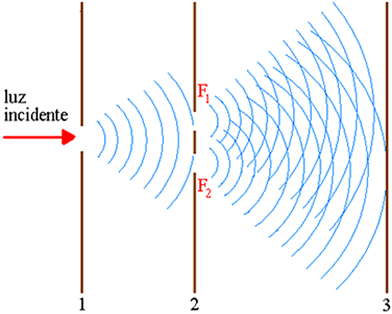
\includegraphics[width=0.6\textwidth]{fenda_dupla.jpg}
    \caption{Esquema experimental do Experimento de Young}
    \label{fig:Young}
\end{figure}
Com isso por meio da difração, as ondas que saem de cada fenda serão ondas circulares e irão interferir com a outra onda emitida pela outra fenda, de forma que isso formará um padrão de interferência no anteparo (parede 3, na figura).
\begin{figure}[H]
    \centering
    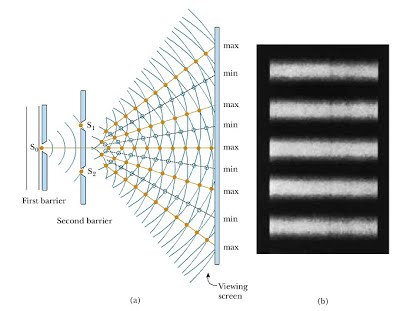
\includegraphics[width=0.8\textwidth]{young_2.jpg}
    \caption{Padrão de interferência do Experimento de Fenda Dupla. As zonas claras são as zonas de interferência construtiva e as zonas escuras são as zonas de interferência destrutiva.}
    \label{fig:young_interferencia}
\end{figure}

Os padrões de interferência são dadas pela geometria dos raios de luz:
\begin{figure}[H]
    \centering
    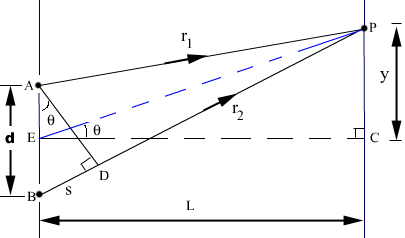
\includegraphics[width=0.6\textwidth]{young1.png}
    \caption{Desenho geométrico dos raios de luz a partir das fendas.}
    \label{fig:geometria_young}
\end{figure}
Lembremos que a difração não altera a fase da onda (se ela antes do buraco é uma crista, após o buraco continuará sendo uma crista). Com isso, as ondas difratadas que saem de A e B tem a mesma fase, ou seja, se a onda que sai de A é uma crista, a onda que sai de B também é.

Perceba que a diferença de tamanho entre $r_1$ e $r_2$ é o segmento $s$. Pela geometria, $s=d\, sen \theta \approx \frac{d y}{L}$. Para que haja interferência construtiva, eu tenho que garantir que, no ponto P, as ondas que venham de $r_1$ e de $r_2$ tenham os suas cristas e vales coincidentes. Porém, para isso acontecer, $s$ tem que ser uma distância múltipla do comprimento de onda, logo:
\begin{equation}
    s= n\lambda = \frac{d}{L}y \quad\quad\quad n=0,1,2,3,...
\end{equation}
\noindent em que $d$ é a distância entre as fendas, $y$ é a altura em relação ao ponto central do anteparo, $L$ é a distância entre as fendas e o anteparo e $\lambda$ é o comprimento de onda.

Para $n=0$, chamamos esse ponto como \textbf{Máximo Central}. Para $n=1$, damos ao ponto o nome de \textbf{Primeira zona de interferência} e assim por diante.

Porém, caso eu queira interferência destrutiva no ponto P, as ondas que venham por $r_1$ e $r_2$ tem que serem um vale e uma crista ou vice-versa (não posso 2 cristas ou 2 vales). Como as ondas que saem das fendas estão em fase, então $s$ tem que ser uma distância múltipla do comprimento de onda da forma $\frac{1}{2}\lambda,\,\frac{3}{2}\lambda,\,\frac{5}{2}\lambda,\,\dots$ para que haja uma crista e um vale para a interferência destrutiva aconteça. Então:
\begin{equation}
    s = \frac{n}{2}\lambda = \frac{d}{L}y \quad\quad\quad n=1,\,3,\,5,\,7,\,\dots
\end{equation}

Dessa forma, acontece o Experimento de Young. Teremos zonas claras intercaladas por zonas escuras, conforme a figura (\ref{fig:young_interferencia}). Também conseguimos montar o gráfico da intensidade de luz em relação à distância ao centro da parede:

\begin{figure}[H]
    \centering
    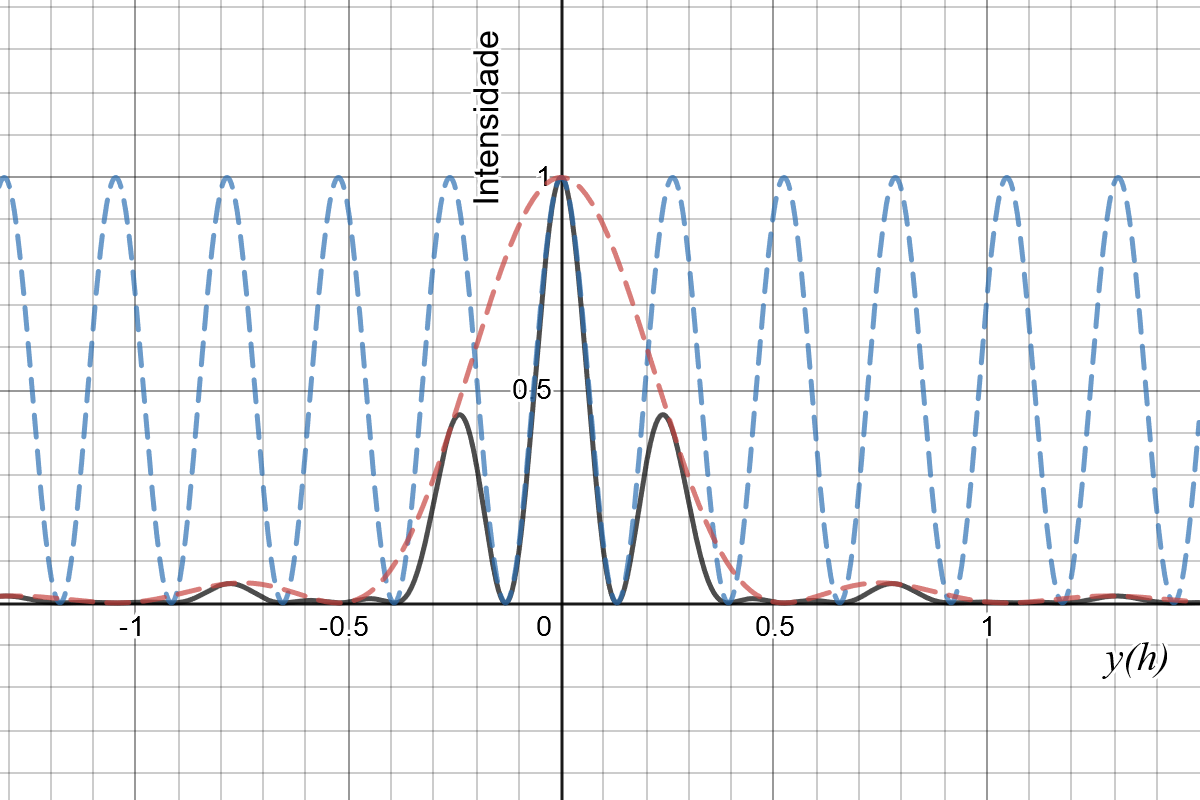
\includegraphics[width=0.9\textwidth]{padrao_inter_difracao.png}
    \caption{Gráfico da intensidade luminosa em relação do experimento de fenda dupla. Em preto está o resultado obtido, em azul está a contribuição da interferência e em vermelho está a contribuição da difração de fenda dupla.}
    \label{fig:resultado}
\end{figure}
Perceba que o resultado é a composição de interferência com a difração e que cada máximo do resultado bate com o máximo da interferência e os mínimos a mesma coisa, exceto para $n=3$, pois para essa caso, o resultado da difração dá 0.

Isso é um resultado somente obtível quando descrevemos a luz como uma onda e isso finalizou a discussão sobre ondas. As equações (1) e (2) descrevem os pontos de interferência construtivas/destrutiva e nos exercícios são essas equações que entram.

\section{Acústica}
A acústica é o estudo sobre ondas sonoras e suas propriedades, muito usada em estúdios, teatros, salas de cinema e de música para que o som nessas salas seja o mais limpo, claro possível e para diminuir ao máximo zonas de interferência destrutiva.

Também usaremos a equação de onda como base das nossos estudos:
\begin{equation}
    v=\lambda f
\end{equation}
\noindent lembrando que $v,\,\lambda,\,f$ são respectivamente a velocidade de propagação da onda, o comprimento de onda e a frequência da onda.

Lembrando que a velocidade de propagação da onda é determinda pelo meio em que a onda se propaga, podemos encontrar a velocidade da onda sonora por meio da seguinte equação:
\begin{equation}
    v=\sqrt{K\,T}
\end{equation}
\noindent em que $v$ é a velocidade de propagação, $K$ é uma constante relacionada ao meio e $T$ é a temperatura do meio em Kelvin (K) (não confundir 'K' da fórmula com o K da unidade Kelvin).

Um detalhe importante sobre a constante $K$ é a seguinte:
\begin{equation}
    K_{gases} < K_{liquidos} < K_{solidos}
\end{equation}
Ou seja, o som se propaga mais rapidamente na água ou no ferro do que no ar. Em geral, a velocidade do som na atmosfera ao nível do mar é:
\begin{equation}
    v_{som} = 343\,m/s = 1237\,km/h
\end{equation}
Quando um avião caça, por exemplo, consegue atingir a velocidades maiores que a velocidade do som, dizemos que \textbf{o avião quebrou a barreira do som.} Isso quer dizer, que veremos o avião se aproximando muito antes de ouvir o seu som. Quando um avião está quebrando a barreira do som, vemos um cone branco ao redor do avião que depois se desfaz a partir do momento que o avião passa da velocidade do som:

\begin{figure}[H]
    \centering
    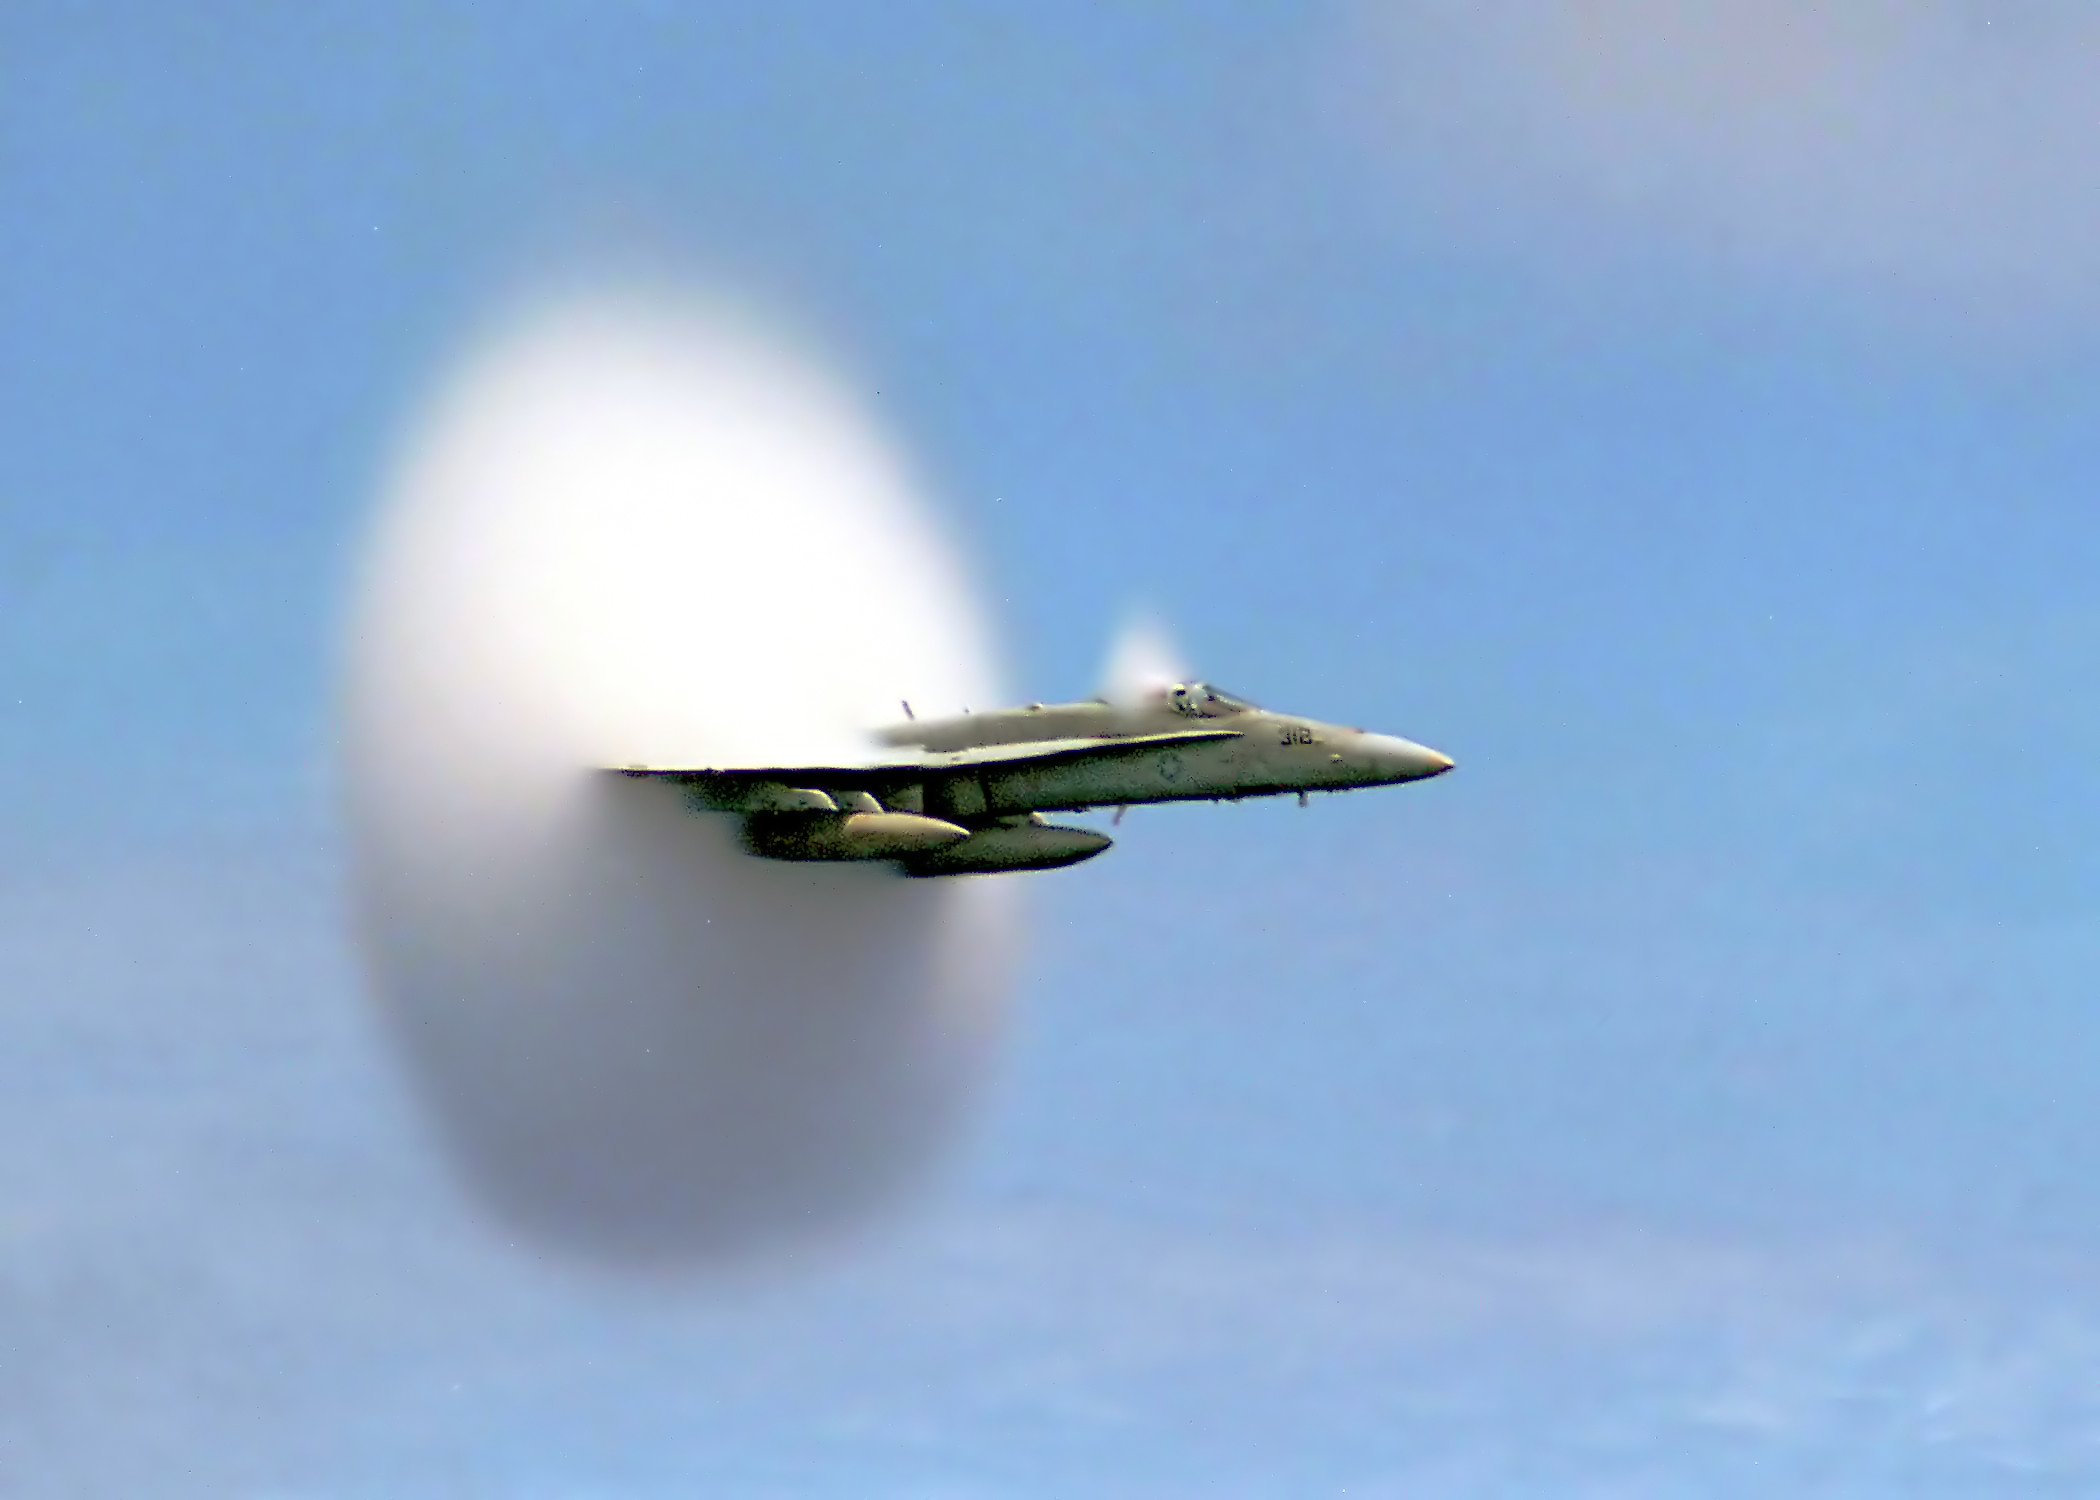
\includegraphics[width=0.6\textwidth]{FA-18_Hornet_breaking_sound_barrier_(7_July_1999)_-_filtered.jpg}
    \caption{Avião caça FA-18 num exercício militar quebrando a barreira do som.}
    \label{fig:barreira do som}
\end{figure}

\subsection{Intensidade sonora e auditiva}
Uma quantidade interessante é o quão forte é uma onda de som em que chamamos de \textbf{Intensidade sonora ($I$)}. Ela é dada por:
\begin{equation}
    I= \frac{P}{A}
\end{equation}
\noindent em que '$P$' é a potência gasta para emitir a onda e '$A$' é a área em que a onda atinge. Essa área irá depender se a onda for bi ou tridimensional (para ondas unidimensionais não tem isso). Para cada um desses casos, temos que:
\begin{itemize}
    \item \textbf{Ondas Bidimensionais (2D)}:
    \begin{equation}
        I = \frac{P}{2\pi\,r}
    \end{equation}
    \noindent em que $r$ é a distância da fonte até a linha em que a onda atinge.
    
    \item \textbf{Ondas Tridimensionais (3D)}:
    \begin{equation}
        I=\frac{P}{4\pi\,r^2}
    \end{equation}
    \noindent em que $r$ é a distância da fonte até o obstáculo em que a onda atinge.
\end{itemize}
Isso é útil para sabermos qual é a distância entre 2 antenas de celulares. No caso dos celulares, as ondas são 3D. O sinal que o nosso celular recebe é a intensidade da onda (I) e pela fórmula, vemos que vamos nos afastando da antena, o sinal fica cada vez mais fraco. Dessa forma, precisamos instalar novas antenas de forma que aumente a área de cobertura.

Uma outra forma usada para analisar intensidade sonora é por meio da \textbf{intensidade auditiva ($\beta$)}. Essa quantidade é definida como:
\begin{equation}
    \beta = 10\,\log_{10}\left(\frac{I}{I_0}\right)
\end{equation}
\noindent em que $I_0$ é a intensidade mínima auditiva: $I_0 = 10^{-12}\frac{W}{m^2}$ e $I$ é a intensidade da onda que ouvimos. \textbf{A intensidade audtiva tem a unidade de decibel $(dB)$}. Em média, sons acima de 120 dB são danosos ao nosso sistema auditivo, podendo até ficarmos surdos. 

Como a fórmula depende do logaritmo da intensidade sonora, para que o som suba por 10 dB, a intensidade sonora ($I$) tem que aumenta por 10 vezes.

Um uso de altos barulhos/sons é usado como forma de atrapalhar os adversários nos mais diversos esportes. Por isso, nos últimos anos, diversos estádios/arenas têm sido construídas de forma que o som vindo das arquibancadas no campo/quadra seja o mais alto possível. 

O recorde mundial atual aconteceu em 2014 no Arrowhead Stadium em Kansas City nos EUA. A torcida do time de futebol americano Kansas City Chiefs fez um barulho de incríveis 142,2 dB durante uma partida de futebol americano. O som é equivalente a estar ao lado de um jato militar, como na foto acima, durante uma decolagem.

No Brasil, não temos esse dado, mas há relatos de ex-atletas que falam sobre o alto barulho da torcida nos estádios como a Vila Belmiro, Arena Corinthians, Mineirão \footnote{tirado do Instituto "Tireidoku"  kkkkkkkkkk, mas acredito que há vários estádios que devem estar nessa lista, isso é só uma brincadeira.}

\subsection{Ondas estacionárias}
Damos o nome de ondas estacionárias o processo de interferência de 2 ondas idênticas se movendo em direções opostas sobre uma corda, dando a impressão de que a onda não se move, que está parada.
\begin{figure}[H]
    \centering
    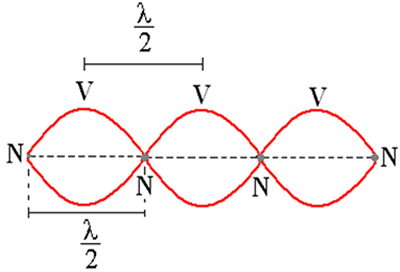
\includegraphics[width=0.6\textwidth]{estacionaria.jpg}
    \caption{Representação de uma onda estacionária}
    \label{fig:estacionaria}
\end{figure}
Os pontos dados pela letra N são os \textbf{nós} e eles estão na posição de repouso da corda. Já os pontos mais altos/baixos da corda são chamados de \textbf{ventres} e são dados pela letra V na imagem (tanto faz ser o ponto mais alto ou o mais baixo). Esses 2 pontos, nó e ventre, são os pontos de interesse de uma onda estacionária.

Uma questão interessante sobre eles é a seguinte: a distância entre 2 nós/ventres consecutivos é metade do comprimento de onda ($d_{V,N} = \lambda/2$, em que $d_{V,N}$ é a distância entre 2 nós consecutivos ou 2 ventres consecutivos). Ou seja, eu preciso passar por 2 ventres/nós para que a distância seja igual à distância do comprimento de onda.

Na próxima aula, veremos a utilidade de trabalhar com ondas estacionárias quando falarmos de tubos, notas musicais e harmônicos.
\end{document}
